\chapter{Background} \label{chap:background}

This section outlines the background information needed to understand the project's scope and clarifies the core concepts that underpin all of the work. We start by defining Hardware Security Modules, followed by a discussion of the technologies that enable the development of a virtualized and distributed version of an HSM. In particular, the main related protocols in the threshold cryptography field and the systems that constitute the basis of our work.


\section{Hardware Security Module} \label{sec:hsm}

A Hardware Security Module (HSM) \cite{hsmdefinition} is a dedicated cryptographic physical device that is specialized in safeguarding the protection of cryptographic keys during their whole life-cycle and performing major cryptographic operations, including generating and securing cryptographic keys, encryption, decryption, strong authentication, and digital signatures, without revealing private-key material to the outside world. HSMs offer a trusted environment that is impenetrable by malware, viruses, exploits, and unauthorized accesses since they are built on top of specialized hardware that is well-tested and certified, have a robust security-focused operating system, restricted network access protected by strict internal rules and firewalls, or are kept off the organization's network to further defend against breaches, causing HSMs to be very difficult, or even impossible, to compromise \cite{hsmpen}. These devices provide efficient and fast automated cryptographic key life cycle tasks, such as random generation, rotation, and protection of keys. Their outstanding performance, when compared with other non-physical solutions, comes from their design, which is optimized for a specific and reduced number of tasks. Figure \ref{fig:hsm-example} represents an example of a general purpose HSM.

There are two main types of HSMs:
\begin{enumerate}
    \item \textbf{General Purpose:} Versatile and adaptable to a wide range of applications, industries, and scenarios. These usually follow well-established specifications, such as PKCS\#11 (or Cryptoki) \cite{pkcs11spec}, which isolate the application from the details of the cryptographic device and enable interoperability between different devices. These are generally used with Public Key Infrastructures, cryptocurrency wallets, and other sensitive data cases. This HSM type is the one this work focuses on.
    
    \item \textbf{Payment and Transaction:} These HSMs are created to protect payment card information and other sensitive transaction information. Although their range of potential use cases is limited, these HSMs are perfect for supporting compliance with Payment Card Industry Security Standards Council (PCI SSC) \cite{pcissc}, one of the significant organizations that produce and maintain standards for HSMs on the banking market.
\end{enumerate}

\begin{figure}[h]
    \begin{center}
        \resizebox{100mm}{!}{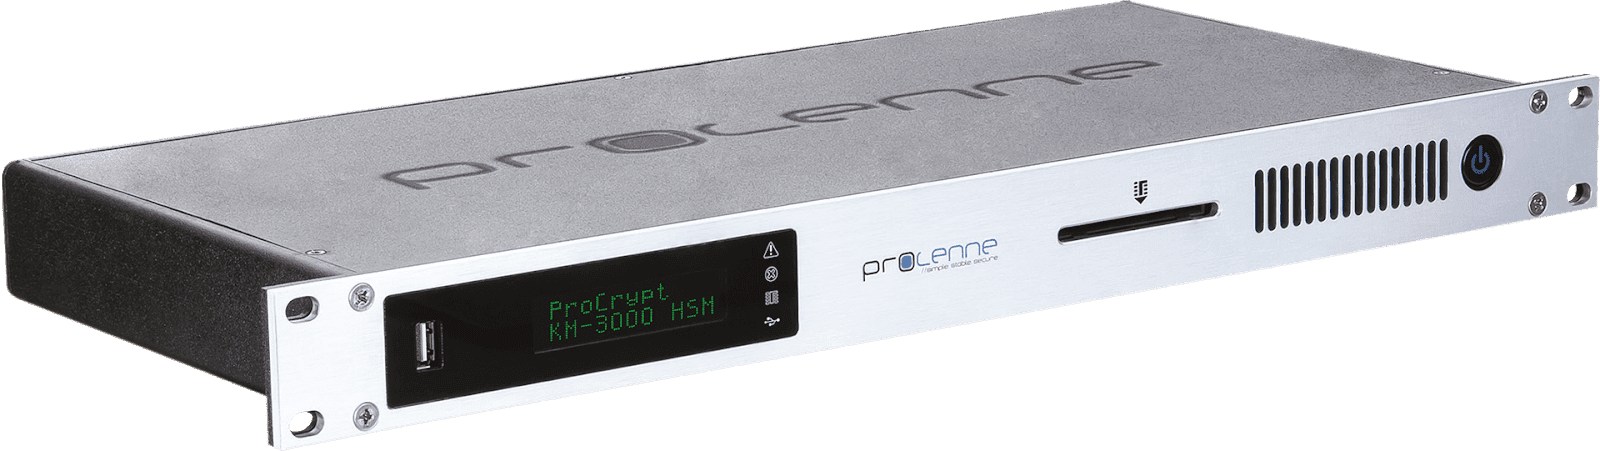
\includegraphics[]{2.hsm-example}}
    \end{center}
    \caption{Example of a General Purpose HSM, ProCrypt KM-3000 \cite{procrypthsm}.}
    \label{fig:hsm-example}
\end{figure}

Due to their crucial role in protecting infrastructures and applications, numerous standards, regulations, and certifications have been established to guarantee that general purpose Hardware Security Modules appropriately safeguard sensitive data and validate the effectiveness of the hardware performing cryptographic operations. Two internationally recognized standards are FIPS 140 \cite{fips140} and Common Criteria \cite{commoncriteria}. The former, Federal Information Processing Standard (FIPS), currently in the third version known as 140-3, is recognized around the world in both the public and private sectors, having four different levels of compliance \cite{fipslevels}, being the Level 3 the most common certification among the HSMs, while in the latter the majority of HSMs are certified at EAL4+, whereas the maximum EAL (Evaluation Assurance Level) is EAL7 \cite{commoncriteriacert}. In financial payment applications, the security of an HSM is frequently verified by comparing it with the standards established by the PCI SSC \cite{pcissc}.

The criteria used by FIPS to classify the effectiveness of the hardware performing cryptographic operations from Level 1 to Level 4 are the following: 
\begin{itemize}
    \item \textbf{Level 1:} The lowest level of security requires production-grade equipment and externally tested algorithms. There are no specific physical security requirements, and attackers can easily access and modify the module.
    \item \textbf{Level 2:} It adds requirements for physical tamper-evidence (the module must have a means of showing evidence of tampering, such as seals or locks) and a role-based authentication mechanism to control access to its services and functions. The module must perform additional self-tests and error handling.
    \item \textbf{Level 3:} A higher level of security than Level 2 that adds requirements for physical tamper-resistance (must have a strong enclosure that resists physical penetration and environmental attacks) and identity-based authentication (a mechanism that verifies the identity of the user or operator). The module must perform more rigorous self-tests and zeroize all sensitive data upon detection of tampering or abnormal conditions. There must also be a physical or logical separation between the interfaces by which critical security parameters enter and leave the module, and private keys can only be imported or exported in their encrypted form.
    \item \textbf{Level 4:} The highest level of security adds requirements for environmental failure protection, fault injection protection, and multi-factor authentication. The module must have a robust enclosure that provides a complete envelope of protection and detects and responds to any unauthorized attempts to gain access (tamper-active); must also protect against fault injection attacks that aim to bypass security mechanisms or induce errors; and implement a multi-factor authentication mechanism that requires the user or operator to present two or more independent factors of authentication, such as something they know, something they have, or something they are.
\end{itemize}

To summarize, the benefits of using Hardware Security Modules include:
\begin{itemize}
    \item compliance with security standards and regulations;
    \item high levels of trust and authentication;
    \item tamper-resistant, tamper-evident, and tamper-active systems to provide extremely secure physical systems;
    \item offering high levels of security for cryptographic keys and sensitive data;
    \item automated cryptographic key life cycle tasks that are fast and efficient, such as random generation, rotation, and protection of keys;
    \item keeping cryptographic keys in one location as opposed to multiple, unknown, and unprotected places;
    \item outstanding performance since it is designed and optimized for a specific and reduced number of tasks. 
\end{itemize}

\subsection{Virtual HSMs} \label{subsec:virtual-hsms}
Virtual Hardware Security Modules are a recent approach to overcome the high costs of these dedicated physical devices and their infrastructure \cite{hsmeconomics}. This alternative has the same responsibilities as the physical devices, including all its benefits, except outstanding performance since HSMs are specialized pieces of hardware and a virtual implementation would need to use other techniques to achieve the same security level we find in common HSMs, penalizing performance, resulting in a trade-off between performance, security, and expenses. These techniques can range from using Trusted Execution Environments (TEEs), such as Intel SGX \cite{intelsgx}, to employing a distributed system and using threshold cryptography to perform the cryptographic operations. Using this last strategy, instead of storing the cryptographic keys in a single location and device, these would be distributed among several servers, each storing a different portion of the original key, resulting in an adversary needing to compromise a determined number of servers to recover the key.


\section{Threshold Cryptography} \label{sec:threshold-cryptography}

Threshold cryptography corresponds to cryptographic algorithms where multiple parties are required to perform cryptographic operations, such as encryptions or signatures, employing a secure distributed protocol that allows the necessary secrets to be used collectively, revealing only the information about the output of the corresponding cryptographic operation. In contrast to depending solely on the security of a single trusted device, this alternative requires that a certain threshold of devices be compromised for an adversary to recover the secrets or violate security, which makes attacks more difficult to execute. Additionally, threshold cryptography is a distributed software-only implementation that aims to achieve at least the same level of security as the algorithms' centralized versions and, in some cases, provide even more security guarantees, namely when using secret sharing for safeguarding cryptographic keys instead of leaving them in a centralized place.

The growing enthusiasm for blockchains such as Bitcoin and Ethereum, the fact that these are moving towards signatures with simpler threshold versions, e.g., Schnorr~\cite{schnorrnotes} and BLS~\cite{blsdraft}, and the recent significant thefts involving the cryptocurrency side of these technologies \cite{cryptothefts2024} are examples that have contributed to reigniting the interest in this subject.  

Threshold cryptography can be divided into three main branches that will be covered next:\textit{ secret sharing}, \textit{threshold signatures}, and \textit{threshold symmetric encryption}.

\subsection{Secret Sharing} \label{subsec:secret-sharing}

A Secret Sharing (SS) scheme protects the confidentiality of the stored data/secret $s$ by splitting it into $n$ pieces, called shares ($s_1...s_n$). To later recover the secret, a portion of its shares must be combined; more specifically, $t + 1 \le n$ of these shares can recover $s$, and $t$ or fewer shares do not reveal any information about the secret. The number of available replicas is represented by $n$, while the maximum number of faulty replicas is symbolized by $t$.

This mechanism plays a vital role in creating a distributed virtual HSM and similar systems since it helps address the issue of securely storing private keys or secrets. Specifically, each replica stores only a share of the secret rather than all the data in clear or encrypted form. As a result, opposite to a single point of failure approach, if a replica is compromised, the adversary can only access the share of that replica, revealing nothing about the original secret.

There are two different major implementations of this scheme:
\begin{itemize}
    \item \textbf{Additive SS}: a simple algorithm where the secret $s$ is added to the remaining shares, corresponding to random values, $s + x_1 + ... + x_n$. Since all shares are required to reconstruct $s$, it can also be called non-threshold SS. This scheme is frequently used in the threshold ECDSA domain \cite{ecdsasurvey}, a threshold signature scheme covered in the next subsection.

    \item \textbf{Shamir SS}: the most popular implementation due to its flexibility in creating more complex schemes. In this scheme \cite{shamir}, the \textit{dealer}, responsible for the distribution of the shares, starts by building a random polynomial $P$ of degree $t$ such that $P(0) = s$ and generates each of the $n$ shares $s_1...s_n$ as points of $P$, $s_i = P(i)$. To recover the secret, the steps involved are: collecting $t + 1$ shares, interpolating the polynomial to recover $P$, and computing $P(0)$.
\end{itemize}

The original scheme, proposed by Shamir, had some limitations in the features it provided and has been improved to strengthen its security throughout the following years. A security aspect not initially available was integrity/verifiability, leaving the scheme vulnerable to active adversaries. This limitation can result in a malicious leader/dealer providing invalid shares or a malicious shareholder corrupting its share, leading the interpolation phase to output a different polynomial $P'$, in which $P'(0)$ will not result in the expected secret. \textit{Verifiable Secret Sharing} (VSS) solves this issue by extending the scheme with commitments. Basically, to each share $s_i$ is added an integrity proof, the commitment $c_i$, that allows shareholders and combiners to detect corrupted shares without revealing any information about the secret. A popular choice for VSS is Feldman's commitment scheme \cite{feldman}, based on exponentiations and the discrete logarithm problem.

As previously stated, secure storage of cryptographic data, such as secrets or private keys, is one of the most critical responsibilities of HSMs. This data type is typically used for extended periods, and over time, an adaptive adversary can corrupt some of the shares. To prevent these scenarios, the \textit{Proactive Secret Sharing} (PSS) scheme \cite{proactivess}, by regularly renewing shares, safeguards the confidentiality of data in long-lived systems against mobile adversaries who can ultimately compromise more than $t$ shareholders.

The aforementioned techniques are both combined in the \textit{Proactive Verifiable Secret Sharing} (PVSS) scheme \cite{pvss} to provide simultaneous share-renewal and verifiability.

Additionally, since these schemes are applied to distributed systems, which are always susceptible to changes in the available servers, alterations to the set of shareholders, including changing servers or even increase/reduce the group size and, consequently, change the threshold value, had to be supported without compromising the confidentiality of the secret. \textit{Dynamic Proactive Verifiable Secret Sharing} (DPVSS) \cite{mpss}, or just DPSS for short, is the term most commonly used to refer to the scheme that also includes this expertise. COBRA~\cite{cobra}, a substantial building block of our system, covered in Section \ref{sec:cobra}, uses it to accomplish confidentiality in BFT SMR systems.

\subsection{Threshold Signatures} \label{subsec:threshold-signatures}

A threshold signature scheme (TSS) enables a group of parties to collectively compute a signature without disclosing any information about their private key. In a $(t, n)$-threshold signature scheme, $n$ parties hold distinct key shares, where any subset of $t + 1 \le n$ distinct parties can issue a valid signature, but a subset of $t$ or fewer parties cannot.

The ultimate goal is to produce signatures in a threshold manner compatible with the existing centralized version of the same signature. In recent years, there has been renewed attention to this topic, primarily due to the development of blockchains. With a threshold signature scheme, the control of a cryptocurrency wallet, which is done through the corresponding private key, is distributed among $n$ servers such that $t + 1$ of them are required to produce a signature; hence, the funds will remain secure even if up to $t$ of these servers are compromised, which makes tampering a signature even more difficult.

With the early adoption of ECDSA in most blockchains, works on developing an efficient threshold version of the signature started to emerge \cite{gennaro18,lindell18,ecdsasurvey}. Nevertheless, ECDSA lacked an efficient way to compress and verify signatures; therefore, a new scheme to improve cryptocurrency scalability, efficiency, and privacy had to be employed. 

Nowadays, the most known and recognized blockchains are converging to a standard of signatures with smaller keys, non-interactive, and linearity schemes, as we can observe by Bitcoin and Ethereum, which began by using ECDSA and recently both received an upgrade where Schnorr and BLS signatures were incorporated, respectively.

Schnorr signatures \cite{schnorrnotes} are provably secure with standard cryptographic assumptions (discrete log), \textit{non-malleable} (a third party cannot alter a valid signature to create another valid one for the same key and message), and provide \textit{linearity}, which allows multiple parties to collaborate in producing a single signature valid for all public keys and enables signers in a multi-signature transaction to combine their public keys into a single aggregated key (key aggregation). Aggregating public keys into a single aggregated signature indistinguishable from a normal one reduces the block load. It also increases privacy since the list and the number of participants will be hidden \cite{schnorradvantages}. In contrast, multi-signature (multi-sig) approaches require each participant to produce an individual signature, which will be individually verified and recorded on-chain. This exposes the number of participants and their public keys, resulting in reduced privacy and an increase in on-chain data. 

BLS signatures \cite{blsdraft} rely on pairing-based cryptography and operate on unique curves, specifically pairing-friendly ones. This signature presents the same advantages as Schnorr, namely, enabling key and signature aggregation. However, the significant downside of BLS signatures is that verification is more inefficient and far more expensive than Schnorr, mainly due to the bilinear-pairing operations \cite{blsbetterthanschnorr}. Nonetheless, the ability to verify many signatures in batches overcomes this issue and can be very attractive for specific applications, particularly blockchains and cryptocurrency systems. 

Schnorr and BLS signatures, due to their linearity scheme, offer several advantages over ECDSA in terms of computational efficiency, storage, and privacy, as well as their simplicity in implementing them in a threshold manner. In contrast to the most recognized and efficient threshold ECDSA implementations, which require 13 communication rounds to complete the signing protocol \cite{lindell18,gennaro18}, or 11 rounds in a recent improvement \cite{gennaro20}, the threshold Schnorr and BLS versions require only two communication rounds to issue their signature.

A well-known implementation of threshold Schnorr signatures is FROST \cite{frost}; its specification was published in a draft standard \cite{frostdraft} and consists of a flexible, round-optimized scheme that minimizes the network overhead of producing Schnorr signatures. This scheme has also been the target of several improvements, both in terms of security and protocol efficiency \cite{frost3,frost3plus}.

Threshold BLS signatures are based on a straightforward combination of secret sharing and group operations and are specified in the IETF BLS signature draft standard \cite{blsdraft}. Tomescu et al. \cite{blsimproved} recently showed that an improvement to the efficiency and performance of the signatures aggregations could be made and proposed an adaptation of well-known fast polynomial interpolation algorithms to accomplish the computations in $O(t*log^2t)$ time, instead of the previous $O(t^2)$.

\subsection{Threshold Symmetric Encryption} \label{subsec:threshold-encryption}

A threshold symmetric encryption (TSE) scheme is a cryptographic operation that secures data by encrypting it in a distributed way, involving multiple participants. In this type of scheme, a predetermined number of participants (the "threshold") must collaborate to recover the original data, either by reconstructing the decryption key or performing a specific algorithm. Unlike traditional symmetric encryption, where a single key is used for both encryption and decryption, TSE ensures that no single entity holds the entire key, preventing unauthorized access even if one party's share is compromised. This approach is particularly useful for secure distributed systems that aim to ensure both confidentiality and resilience against attacks.

Multiple threshold cryptography schemes have been developed based on public-key cryptography, whereas symmetric-key schemes have not received the same focus and attention, leaving important security concerns and efficiency challenges to be resolved. Desirable features like each participant providing auxiliary data that can be used to check its partial result are supported in some threshold asymmetric cryptography schemes; however, symmetric-key encryption schemes, such as AES, do not offer this property due to the different nature of symmetric ciphers' algebraic structures.

A simple but insecure way of implementing threshold symmetric encryption is using secret sharing on the key of the authenticated encryption scheme, such as AES-GCM \cite{aesgcm}, where the key shares are sent to multiple parties, and then one of them reconstructs it to perform the encryption or decryption operation. Nevertheless, reconstructing the key negates the benefits of splitting it in the first place. Another approach would be to apply the secret sharing scheme directly to the plaintext instead of the key. While this avoids key reconstruction, it significantly increases communication and storage costs. Likewise, using secure multi-party computation (MPC) could be a possibility since it would allow keys to remain split during the operations, but it would also have a significant performance cost due to the required multiple rounds of high bandwidth communication between the parties. Therefore, high performance and efficiency can only be achieved by creating a dedicated threshold authenticated encryption algorithm.

The most recognized and well-known proposal for a threshold symmetric encryption scheme is DiSE~\cite{dise}. It presents the first formal treatment for \textit{Distributed Symmetric-key Encryption} (DiSE), which presents new notions of correctness, privacy, and authenticity in the presence of malicious attackers. The proposal consists of a generic construction of \textit{threshold authenticated encryption} (TAE) based on any distributed pseudorandom function (DPRF).

A DPRF is a distributed and interactive analog of a standard PRF. It is the main building block of DiSE, allowing a threshold number of distributed parties to collectively evaluate a function without reconstructing the shared secret. Initially, it involves a setup where each party obtains their share from a secret and the public secret sharing parameters. The DiSE and, in consequence, the DPRF start their protocol after receiving a commitment of the message to be encrypted sent by the client (or also called \textit{encryptor} or \textit{evaluator}). This input is collectively evaluated during the DPRF by any $t$ parties where $t$ ($\le n$) is a threshold. At the end of the DPRF protocol, only one party, the \textit{encryptor}, learns the output, a partial result sent by multiple parties that allows the \textit{encryptor} to assemble the final ciphertext and complete the DiSE algorithm. 

The chosen DPRF algorithm should meet two main requirements: (i) \textit{consistency}: the evaluation should be independent of the participating set, (ii) \textit{pseudorandomness}: the evaluation's output should be pseudorandom to everyone but the evaluator even if an adversary corrupts all other $t - 1$ parties and behaves maliciously. In this malicious case, a stronger property must be applied, (iii) \textit{correctness}: after an evaluation involving up to $t - 1$ malicious corruptions, an honest evaluator either receives the correct output or can detect the malicious behavior. Naor et al. \cite{naor} proposed and developed two very efficient two-round instantiations of DPRF, one based only on symmetric-key cryptography and another based on the Decisional Diffie-Hellman (DDH) assumption \cite{ddh}, being both used to provide the first formal proof of security for these constructions under a strong pseudorandomness requirement in DiSE.

In DiSE, the primary responsibility of the DPRF is to generate a pseudorandom key $w$ to encrypt the message $m$. For an adversary not to be able to reuse $w$ to create more than one valid ciphertext, the input provided to the DPRF is the identity of party $j$ concatenated with the message $m$, ($j||m$). 
This way, by placing $j$ inside the DPRF, a malicious attacker can not obtain $w$ by replacing the input of the DPRF in a new encryption query and thereby can not recover any message encrypted by an honest encryptor. Although the protocol checks for each party if a message $(j, \ast)$ comes from party $j$, this strategy reveals $m$ to all other parties, failing to achieve message privacy and efficient communication cost. To overcome this issue, a commitment of $m$ is sent to the DPRF. The hiding and binding property of the commitment ensures that $m$ remains secret and that $w$ is bound to this particular message. Nevertheless, the attacker could still generate valid ciphertexts by keeping $m$, $j$, and $w$ the same and using new randomness to encrypt $m$. This is prevented by making the ciphertext deterministic given $m$ and $w$: $w$ serves as input to a pseudorandom number generator (PRNG) to produce a pseudorandom string serving as a \textit{"one-time pad"} that is used to encrypt $m$ through an exclusive-OR (XOR) operation. 

Using an analogy with threshold signatures and using Figure \ref{fig:dise-simple-algo} as reference, the DPRF, for each server, will produce a deterministic partial result $k_i$, which the corresponding client that made the request will have the responsibility of aggregating them into the final ciphertext $c$ using the combined partial results $k$, with the desired message $m$ that was never shared with any of the available servers, but only a commitment of it, $t$.

\begin{figure}[h]
    \begin{center}
        \resizebox{120mm}{!}{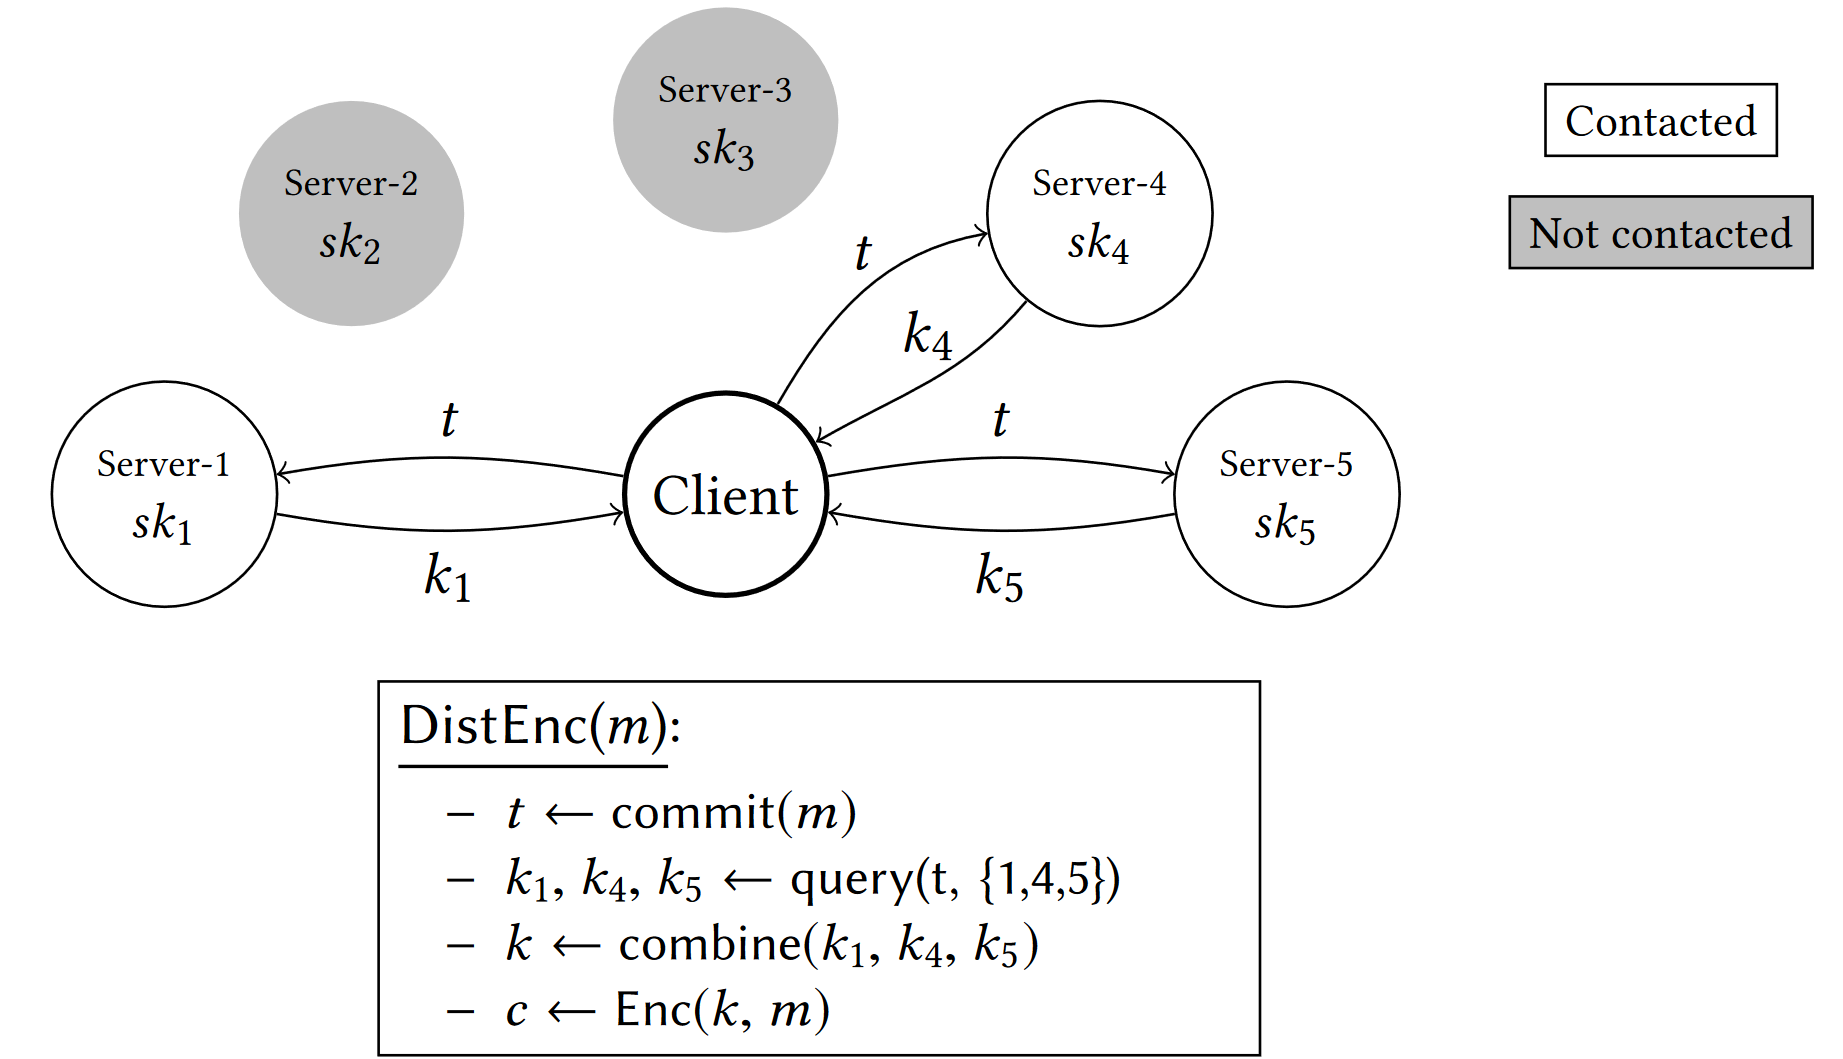
\includegraphics[]{2.dise-simple-algo}}
    \end{center}
    \caption{DiSE simplified protocol for $n=5$ and $t=3$ \cite{dise}.}
    \label{fig:dise-simple-algo}
\end{figure}

The DiSE protocol is composed of the following steps:
\begin{enumerate}
    \item Generate and distribute random symmetric keys to the $n$ servers;
    \item Upon receiving an \textbf{encryption} request from a client, any of the servers (say server $j$) can act as the \textit{initiator} (or \textit{encryptor}) to invite other ($t - 1$) servers to encrypt a message $m$ as follows:

    \begin{enumerate}
        \item Server $j$ first generates a long random number $\rho$ and calculates $\alpha = h(m \| \rho)$, where $h$ is a cryptographic hash function and $||$ denotes string concatenation;
        \item  Server $j$ chooses ($t - 1$) other active servers, sends ($j \| \alpha$) to them over secure channels, and asks them to return partial results $w_i$, so that $j$ can combine them into $w = \mathsf{DPRF}(j \| \alpha)$;
        \item Server $j$ assembles the final ciphertext $c = (c_1, j, \alpha)$, using a $\mathsf{PRNG}$, i.e., a pseudorandom number generator, where $c_1 = \mathsf{PRNG}(w) \oplus (m \| \rho)$.
    \end{enumerate}
    
    \item To perform the \textbf{decryption} operation, server $i$ agrees to act as the \textit{initiator}, or \textit{decryptor}, to decrypt a received ciphertext $c' = (c_1', j', \alpha')$, which may or may not be $c$ due to possible modification attacks.

    \begin{enumerate}
        \item Server $i$ chooses ($t - 1$) other active servers, which calculate $w' = \mathsf{DPRF}(j' \| \alpha')$, collectively;
        \item Server $i$, after receiving the necessary responses, computes $c' \oplus \mathsf{PRNG}(w')$ and parses the result into ($m' \| \rho'$);
        \item In the end, server $i$ checks the validity of the plaintext by verifying whether $\alpha' = h(m' \| \rho')$. If they do not match, ciphertext $c'$ has been tampered with and will be rejected.
    \end{enumerate}
\end{enumerate}

DiSE has been the subject of continued studies in the years that followed its publication, mainly due to the novelty and remarkable improvements made in the threshold symmetric-key encryption field, where the improvements were focused on the security guarantees and definitions, rather than changing the basis of the previously described protocol. 

\textit{Amortized Threshold Symmetric-key Encryption} (ATSE) \cite{amortizeddise} was one of the first works to provide improvements to the initial DiSE proposal. This work proposes a new primitive, formalized as \textit{flexible threshold key-derivation} (FTKD), to counter the necessity for interaction on each invocation of DiSE, which limits performance and incurs heavy computations and communication on the servers when encrypting large datasets.

\textit{Robust DiSE} \cite{robustdise}, on the other hand, intends to enhance the system's robustness by eliminating the honest-initiator assumption, introducing a rotating initiator role among active servers, and statistically detecting any attempt to use a compromised server repeatedly as the initiator, blocklisting the corresponding server.

\textit{ParaDiSE} \cite{paradise} is a recent proposal where Agrawal and other authors of the initial protocol revisit the problem of designing secure and efficient threshold authenticated encryption schemes. This work introduced new TAE security definitions to fix the issues found in the original DiSE proposal, namely definitions for capturing confidentiality, integrity, and preventing key reconstruction. In this new proposal, the authors departed from a more abstract description of TAE schemes and focused only on those operating in two communication rounds.

\section{State Machine Replication Systems} \label{sec:smr}

A state machine replication (SMR) system \cite{smr} is a strategy used in distributed computing to ensure that a group of replicas maintain the same state and perform the same operations in a deterministic and coordinated manner, i.e., in the same order, leading to consistent states across all replicas. This approach is crucial for building reliable fault tolerance and highly available distributed systems.

Distributed systems intended for real-world scenarios must use this approach combined with an effective and realistic fault model. The system we propose in this dissertation, a distributed and virtual HSM, must employ a Byzantine fault-tolerant SMR system since it is the classical method for implementing consistent and fault-tolerant services. This approach maintains the integrity and availability of a secure service, even if a fraction of the replicas fail in a Byzantine way. Instead of using a \textit{Crash Fault-Tolerant (CFT)} model, in which the fault would occur when a replica is faulty, that is, the system stops working or fails to respond, a \textit{Byzantine Fault-Tolerant (BFT)} model takes into account that a replica can behave arbitrarily or maliciously, sending incorrect or conflicting messages to other replicas in the system. This type of fault is more realistic and more challenging to detect and recover from because a faulty replica may try to deceive the others, causing the system to behave in unexpected ways, leading to inconsistencies and probably security vulnerabilities.

To avoid these issues, BFT SMR protocols are designed to tolerate these faults by ensuring that a correct replica can always progress despite the presence of faulty replicas. This is achieved through a consensus-based approach that requires a certain number of replicas to agree on the order of the commands to be executed. Another critical aspect of the underlying model of this type of system is communication \cite{commsmodel}.
In a \textit{synchronous communication model}, the messages are assumed to be delivered within a known and bounded time frame, simplifying the protocol design since it allows replicas to agree on the order of the commands even in the presence of Byzantine faults. However, this assumption is unrealistic in practice because network delays and failures are constantly occurring and can cause messages to be delayed or lost.
In contrast, in an \textit{asynchronous model}, the system assumes that messages can be arbitrarily delayed or lost, requiring more complex mechanisms to achieve consensus among replicas despite the presence of Byzantine faults.
Nevertheless, \textit{partially synchronous communication} \cite{partiallysynchronous} is the preferred model due to its realism and practicality. It accommodates real-world variability in message and processing delays by combining elements of synchronous and asynchronous models. This model ensures the eventual delivery of messages within certain bounds without requiring strict adherence to those bounds at all times, given that network and processes may behave asynchronously until some \textit{unknown} global stabilization time ($\mathsf{GST}$), which then become synchronous. This allows the system to handle temporary delays and network partitions while maintaining system performance and reliability. Algorithms designed for this model can optimize operations during synchronous periods and ensure safety and liveness during asynchronous periods. 

Examples of recognized works that produced protocols in the partially synchronous system model are Paxos \cite{paxos} and Raft \cite{raft}, protocols that solve consensus for CFT SMR systems, and also PBFT \cite{pbft} and BFT-SMaRt \cite{bftsmart}, which instead use the BFT model. PBFT was the first BFT protocol to achieve a performance similar to its CFT counterparts. BFT-SMaRt implements a library with a similar algorithm to PBFT that allows protocols that require a robust BFT SMR model to extend and use its functionalities, as is the example of COBRA, which is covered next.



\section{COBRA} \label{sec:cobra}

COBRA (COnfidential Byzantine ReplicAtion) \cite{cobra} implements confidentiality in practical BFT SMR systems through a new protocol stack for Dynamic Proactive Secret Sharing (DPSS). This framework, achieves high levels of security, consistency, robustness, fault-tolerance, integrity, and availability, and is an ideal candidate to be used underneath distributed systems that require these kinds of properties. COBRA did not directly develop some of these characteristics, but inherited from the library upon which it was built, BFT-SMaRt \cite{bftsmart}, a popular open-source BFT SMR library that provides essential BFT SMR features to the systems that extend it, including fault and asynchrony tolerance, crash recovery, and group reconfiguration.

Previous works that tackled the confidentiality issue in BFT SMR systems addressed the problem by integrating secret sharing with the consensus-based framework of BFT SMR. However, they did not provide several important capabilities for this type of system, such as replica recovery, group reconfiguration, and acceptable performance when handling a large number of secrets. Certain works, such as DepSpace \cite{depspace}, started using threshold cryptography, namely Verifiable Secret Sharing (VSS), to protect the confidentiality of stored data, providing a confidentiality layer for practical BFT SMR services. Nevertheless, those works did not consider adaptive mobile adversaries and adaptive sets of shareholders.

COBRA addressed these limitations with a novel approach for proactive verifiable secret sharing in dynamic groups of processes. The modular protocol stack consists of three main components: \textit{distributed polynomial generation}, \textit{share recovery}, and \textit{dynamic secret resharing}, represented in Figure \ref{fig:2.cobra-protocol-stack}. Together, these ensure that sensitive data is protected from adversaries and that the system can recover from failures without compromising confidentiality.

\begin{figure}[h]
    \begin{center}
        \resizebox{100mm}{!}{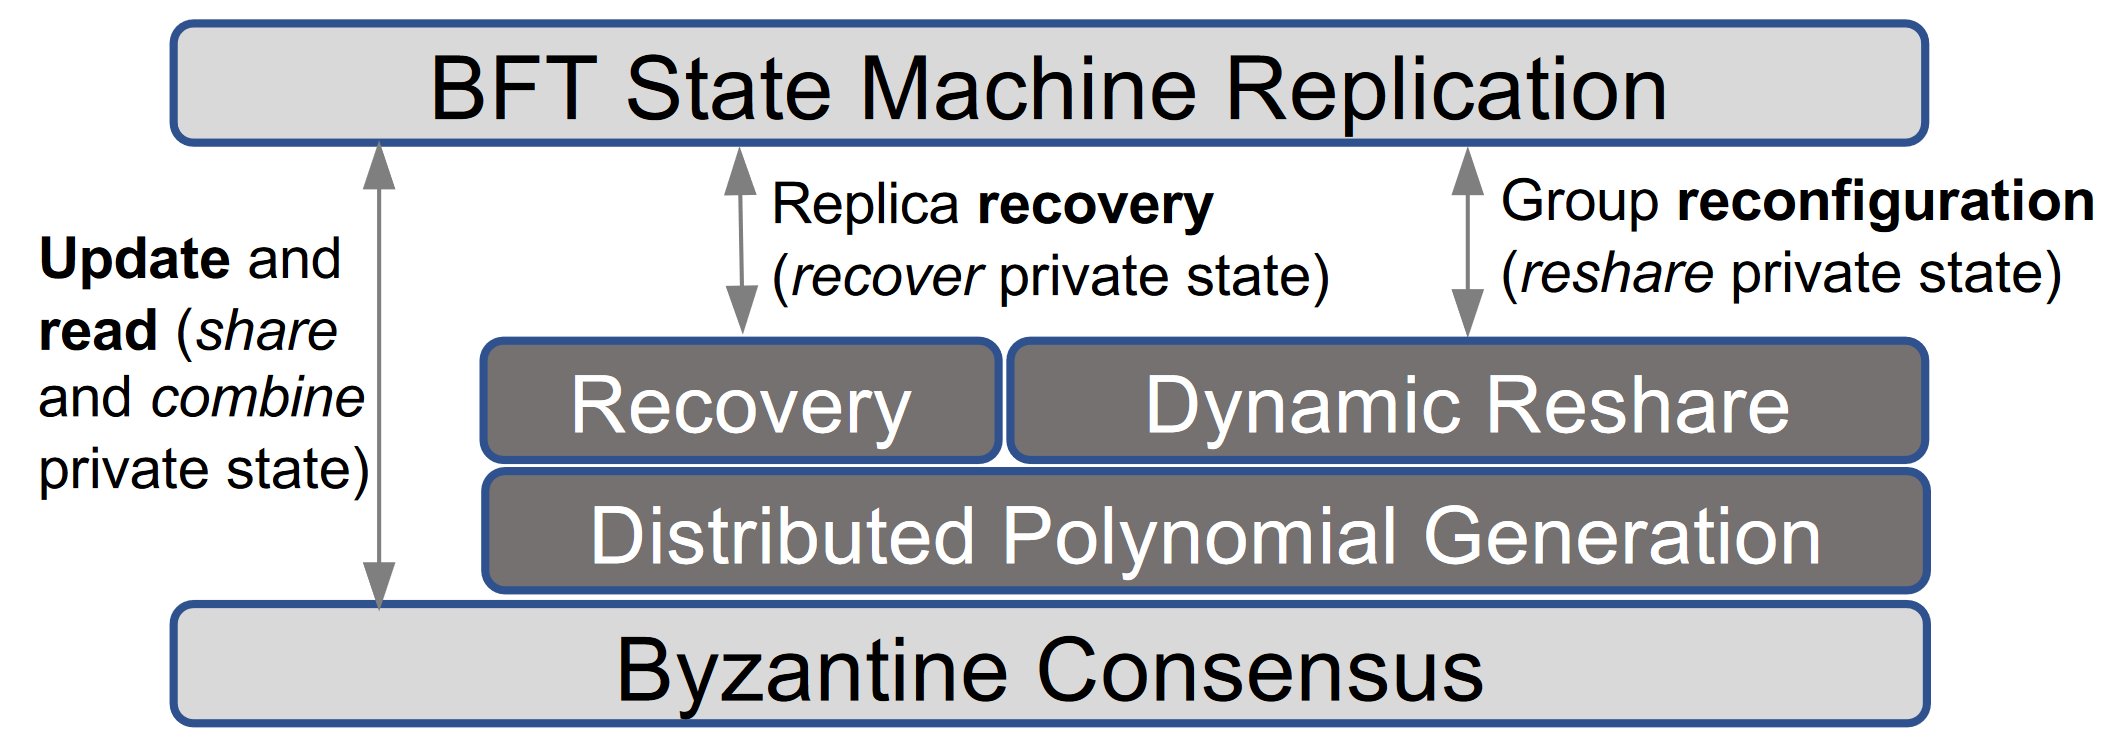
\includegraphics[]{2.cobra-protocol-stack}}
    \end{center}
    \caption{COBRA DPSS protocol stack represented by dark boxes \cite{cobra}.}
    \label{fig:2.cobra-protocol-stack}
\end{figure}

Furthermore, COBRA uses Byzantine consensus for \textit{distributed polynomial generation}. The distributed polynomial generation protocol allows replicas to jointly create new random and secret polynomials in a distributed way, with shares distributed to at least $t + 1$ correct servers, which is enough for their reconstruction. These polynomials serve as a basis for other protocols in the system stack: replica recovery, secret resharing, and group reconfiguration. To ensure the liveness of the consensus protocol employed, the authors assume a partially synchronous model \cite{partiallysynchronous} in which the network and processes may behave asynchronously until some \textit{unknown} global stabilization time ($\mathsf{GST}$), then become synchronous. To avoid some executions being adversary-influenced, the \textit{share recovery} requires $t + 1$ correct servers to rebuild the replica state, and the \textit{secret reshare} requires that all servers obtain valid renewed shares. This is done by the recovery protocol, which can identify and remove the processes that caused the generation of invalid shares during polynomial generation. This results in the correct servers re-executing the recovery protocol and ignoring messages from removed faulty servers, where eventually only correct servers participate.

Supporting replica recovery requires the re-generation of the replica's lost shares. When a server $r_i$ recovers from a failure, it needs (1) to obtain the common part \textit{C} of its state (which is replicated on other servers) using a state transfer protocol and (2) invoke the share recovery protocol for each stored data entry $D_j$, effectively reconstructing its private state. Regarding the state of the system, the \textit{Confidential SMR} service model contains a global system state \textit{S}, and locally each replica maintains two states, one common to all replicas \textit{C}, and one specific to each replica, containing the replica shares. The former is composed of $C = \{\langle\overline{D}_1, D^e_1, c_1\rangle, ..., \langle\overline{D}_m, D^e_m, c_m\rangle\}$: $\overline{D}_j$ is the non-sensitive data associated with the data entry (e.g., the key of a stored value, the metadata of a transaction in a blockchain), $D^e_j$ represents the data encrypted, and $c_j$ is the commitment for the shares of the encryption key. The private state of the replica contains the shares of the corresponding keys.

The COBRA paper presents an experimental evaluation of the system, considering up to 97 replicas and a state containing 100,000 stored secrets, showing that it is significantly faster than existing related work, for instance, resharing this number of secrets in a group of ten servers would require less than 12 minutes, which is, according to the authors, five times faster than Mobile Proactive Secret Sharing (MPSS) \cite{mpss}, a state-of-the-art protocol that uses a different technique to achieve DPSS.

Besides the critical features for practical BFT SMR systems inherited from BFT-SMaRt and the implementation of confidentiality in this type of system, allowing the secure storage of a large number of secrets, COBRA also supports replica recovery, secret resharing, share recovery, and group reconfigurations.

\section{Final Remarks} \label{sec:background-final-remarks}

This chapter started by identifying what hardware security modules are, specifically describing their main functionalities, responsibilities, and benefits, ending with a comparison between physical and virtual HSMs, highlighting their main differences. Next, we presented the main technologies that allow us to implement the system we propose in this dissertation, a virtual and distributed HSM that uses only software to develop and perform cryptographic operations. These technologies include threshold cryptography, namely, secret sharing, threshold signatures, and threshold symmetric encryption, followed by clarifying the concepts behind the systems we use underneath our implementation, that is, the BFT SMR system, which allows our project to be realistic and practical in the real world, and COBRA, a novel framework that added confidentiality to this type of system efficiently and securely.

\LIMPA